\documentclass[aspectratio=169,11pt]{beamer}
\usetheme{Madrid}
\usecolortheme{default}
\usepackage[T1]{fontenc}
\usepackage{amsmath,amssymb,booktabs,array}
\usepackage{tikz,pgfplots}
\pgfplotsset{compat=1.18}
\usepackage{listings}
\usepackage{xcolor}
\definecolor{codebg}{RGB}{245,247,249}
\lstset{language=Python,basicstyle=\ttfamily\scriptsize,backgroundcolor=\color{codebg},frame=single,breaklines=true,showstringspaces=false,columns=fullflexible,keepspaces=true}
\title[Binary ROC curves]{From the Confusion Matrix to the ROC Curve}
\subtitle{Binary classification: a practical, reproducible construction}
\author{Morten Hjorth-Jensen}
\date{\today}
\begin{document}
\begin{frame}\titlepage\end{frame}
\begin{frame}{The central idea}
\begin{block}{One confusion matrix gives one ROC point}
For a fixed classification threshold $t$, a confusion matrix determines one pair $(\mathrm{FPR}(t),\mathrm{TPR}(t))$.
\end{block}
\begin{itemize}
\item A \emph{full} ROC curve requires varying $t$ across the classifier's scores.
\item Keep the true test labels $y_i$ and the continuous positive-class scores $s_i$.
\item Retraining is unnecessary: only the decision rule changes. Use your final model and call it with different threesholds $t$ for the say the sigmoid function which outputs the final value.
\end{itemize}
\end{frame}
\begin{frame}{Binary confusion matrix}
\centering
\begin{tabular}{lcc}
\toprule
& Predicted positive & Predicted negative\\\midrule
Actual positive & TP & FN\\
Actual negative & FP & TN\\\bottomrule
\end{tabular}
\vspace{1em}
\begin{align*}
\mathrm{TPR}&=\frac{\mathrm{TP}}{\mathrm{TP}+\mathrm{FN}}, &
\mathrm{FPR}&=\frac{\mathrm{FP}}{\mathrm{FP}+\mathrm{TN}},\\
\mathrm{TNR}&=\frac{\mathrm{TN}}{\mathrm{TN}+\mathrm{FP}}, &
\mathrm{FNR}&=\frac{\mathrm{FN}}{\mathrm{FN}+\mathrm{TP}}.
\end{align*}
\small $\mathrm{TPR}=1-\mathrm{FNR}$ and $\mathrm{FPR}=1-\mathrm{TNR}$.
\end{frame}
\begin{frame}{What must be saved from the final classifier?}
For each held-out test observation $i$, retain
\begin{equation*}
y_i\in\{0,1\},\qquad s_i\in\mathbb{R},
\end{equation*}
where $s_i$ is a score increasing with confidence in class 1 (often $s_i=P(y_i=1\mid\mathbf{x}_i)$).
\begin{block}{Threshold rule}
\[\widehat y_i(t)=\begin{cases}1,&s_i\ge t,\\0,&s_i<t.\end{cases}\]
\end{block}
A sigmoid probability, neural-network logit, SVM decision score, or tree-ensemble probability can be used. Calibrated probabilities are \emph{not} required.
\end{frame}
\begin{frame}{Eight test observations: a worked example}
\centering
\begin{tabular}{c*{8}{c}}
\toprule
Observation $i$ &1&2&3&4&5&6&7&8\\\midrule
True $y_i$ &1&0&1&1&0&0&1&0\\
Score $s_i$ &.95&.85&.75&.65&.55&.45&.35&.15\\\bottomrule
\end{tabular}
\vspace{1em}
At $t=0.50$, the predicted classes are
\[\widehat{\mathbf y}=(1,1,1,1,1,0,0,0).\]
Thus $\mathrm{TP}=3$, $\mathrm{FP}=2$, $\mathrm{FN}=1$, $\mathrm{TN}=2$, giving
\[\boxed{(\mathrm{FPR},\mathrm{TPR})=(2/4,3/4)=(0.50,0.75).}\]
\end{frame}
\begin{frame}{Sweep the threshold: construct a family of matrices}
\centering\small
\begin{tabular}{lrrrrrr}
\toprule
Threshold $t$ & TP & FP & FN & TN & TPR & FPR\\\midrule
$t>.95$ &0&0&4&4&0&0\\
$.95$ &1&0&3&4&.25&0\\
$.85$ &1&1&3&3&.25&.25\\
$.75$ &2&1&2&3&.50&.25\\
$.65$ &3&1&1&3&.75&.25\\
$.55$ &3&2&1&2&.75&.50\\
$.45$ &3&3&1&1&.75&.75\\
$.35$ &4&3&0&1&1.00&.75\\
$.15$ &4&4&0&0&1.00&1.00\\\bottomrule
\end{tabular}
\vspace{.5em}
\small Every row supplies one ROC coordinate $(\mathrm{FPR}(t),\mathrm{TPR}(t))$.
\end{frame}
\begin{frame}{The ROC curve for the eight observations}
\centering
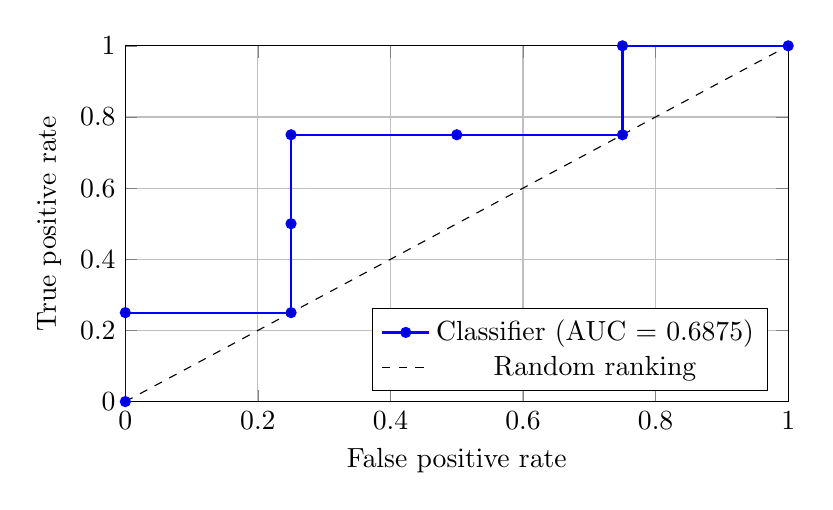
\begin{tikzpicture}
\begin{axis}[width=10cm,height=6.1cm,xmin=0,xmax=1,ymin=0,ymax=1,xlabel={False positive rate},ylabel={True positive rate},grid=major,legend pos=south east]
\addplot+[const plot,thick,mark=*,mark size=1.6pt] coordinates {(0,0) (0,.25) (.25,.25) (.25,.50) (.25,.75) (.50,.75) (.75,.75) (.75,1) (1,1)};
\addlegendentry{Classifier (AUC = 0.6875)}
\addplot[dashed,black,domain=0:1,samples=2] {x};
\addlegendentry{Random ranking}
\end{axis}
\end{tikzpicture}
\end{frame}
\begin{frame}{Why the curve is step-shaped}
\begin{itemize}
\item Lowering $t$ past a \emph{positive} example increases TP and TPR, giving a vertical step.
\item Lowering $t$ past a \emph{negative} example increases FP and FPR, giving a horizontal step.
\item With tied scores, several examples can enter at once; both rates may change together.
\item Thresholds above the maximum score and at or below the minimum score give the endpoints $(0,0)$ and $(1,1)$.
\end{itemize}
\begin{block}{ROC axes}
\[x=\mathrm{FPR}(t),\qquad y=\mathrm{TPR}(t).\]
\end{block}
\end{frame}
\begin{frame}{Only a final confusion matrix?}
Suppose the only stored result is
\[C=\begin{pmatrix}\mathrm{TN}&\mathrm{FP}\\\mathrm{FN}&\mathrm{TP}\end{pmatrix}=\begin{pmatrix}80&20\\10&90\end{pmatrix}.\]
Then
\[\mathrm{FPR}=\frac{20}{80+20}=0.20,\qquad \mathrm{TPR}=\frac{90}{90+10}=0.90.\]
\begin{alertblock}{Important limitation}
The matrix supplies the point $(0.20,0.90)$, but \emph{not} the entire ROC curve. Recover the individual test scores from the trained model.
\end{alertblock}
\end{frame}
\begin{frame}{AUC: interpretation}
\begin{block}{Ranking probability}
For an independently drawn positive score $S_+$ and negative score $S_-$,
\[\mathrm{AUC}=P(S_+>S_-)+\tfrac12P(S_+=S_-).\]
\end{block}
\begin{itemize}
\item $\mathrm{AUC}=1$: all positive observations rank above negatives.
\item $\mathrm{AUC}=0.5$: random ranking performance.
\item $\mathrm{AUC}<0.5$: scores tend to rank classes in reverse order.
\item Example: $\mathrm{AUC}=11/16=0.6875$ (11 correctly ordered positive--negative pairs out of 16).
\end{itemize}
AUC is not a measure of probability calibration and does not choose a decision threshold.
\end{frame}
\begin{frame}[fragile]{NumPy implementation: compute ROC points}
\begin{lstlisting}
import numpy as np

y_true = np.array([1, 0, 1, 1, 0, 0, 1, 0])
y_score = np.array([.95, .85, .75, .65,
                    .55, .45, .35, .15])

thresholds = np.r_[np.inf,
                   np.sort(np.unique(y_score))[::-1]]
fpr, tpr = [], []

for t in thresholds:
    pred = (y_score >= t)
    tp = np.sum((y_true == 1) & pred)
    fn = np.sum((y_true == 1) & ~pred)
    fp = np.sum((y_true == 0) & pred)
    tn = np.sum((y_true == 0) & ~pred)
    tpr.append(tp / (tp + fn))
    fpr.append(fp / (fp + tn))
\end{lstlisting}
\end{frame}
\begin{frame}[fragile]{NumPy and Matplotlib: plot ROC and AUC}
\begin{lstlisting}
import matplotlib.pyplot as plt

# fpr and tpr come from the preceding slide.
auc = np.trapezoid(tpr, fpr)  # NumPy 2.0+
# For older NumPy versions, use np.trapz(tpr, fpr).

plt.figure(figsize=(7, 5))
plt.plot(fpr, tpr, '-o', label=f'ROC (AUC={auc:.4f})')
plt.plot([0, 1], [0, 1], 'k--', label='Random ranking')
plt.xlabel('False positive rate')
plt.ylabel('True positive rate')
plt.xlim(0, 1)
plt.ylim(0, 1)
plt.grid(True)
plt.legend()
plt.show()
\end{lstlisting}
\end{frame}
\begin{frame}{Practical workflow and evaluation discipline}
\begin{enumerate}
\item Train the classifier using training data.
\item Use validation data for model selection and threshold tuning. This is next week's exercise. Use here only the trained model, no cross-validation
%\item Evaluate \emph{once} on held-out test data; retain $(y_i,s_i)$ for every observation.
\item Sort the distinct scores and sweep thresholds from high to low.
\item Compute TP, FP, FN, TN, then TPR and FPR at each threshold.
\item Plot the ROC points and compute AUC.
\end{enumerate}
\begin{block}{Take-home message}
A ROC curve is a \emph{family of confusion matrices} for one trained model, indexed by the decision threshold.
\end{block}
\end{frame}
% Appended multiclass section. All preceding binary slides are preserved.
\section{Multiclass classification: MNIST}
\title[Multiclass ROC curves]{From the Confusion Matrix to the ROC Curve}

\begin{frame}{From binary classification to MNIST}
\begin{block}{Ten classes, ten scores per image}
For MNIST, $y_i\in\{0,1,\ldots,9\}$. Keep the true label and the
\emph{entire} score vector for every held-out image:
\[
  \mathbf s_i=(s_{i0},\ldots,s_{i9}),\qquad
  S\in\mathbb R^{N\times10},\qquad Y_{ik}=\mathbf1\{y_i=k\}.
\]
\end{block}
\begin{itemize}
\item A softmax network supplies estimates $s_{ik}=\widehat P(y_i=k\mid\mathbf x_i)$,
      with $\sum_k s_{ik}=1$.
\item The final class prediction is $\widehat y_i=\arg\max_k s_{ik}$.
\item ROC evaluation uses \emph{scores}, not only these argmax predictions.
\item There is no unique multiclass ROC curve: specify the binary reduction
      and averaging convention.
\end{itemize}
\end{frame}

\begin{frame}{The $10\times10$ confusion matrix}
\small
Rows are true digits; columns are predicted digits:
\[
 C_{ab}=\sum_{i=1}^{N}\mathbf1\{y_i=a,\widehat y_i=b\},
 \qquad a,b\in\{0,\ldots,9\}.
\]
\centering
\setlength{\tabcolsep}{6pt}
{\footnotesize
\begin{tabular}{c|rrrrrrrrrr}
\toprule
True $\backslash$ predicted & 0&1&2&3&4&5&6&7&8&9\\\midrule
0&96&0&0&0&0&1&1&0&2&0\\
1&0&98&0&0&0&0&0&1&1&0\\
2&1&1&94&1&0&0&0&1&2&0\\
3&0&0&1&93&0&3&0&1&1&1\\
4&0&0&0&0&95&0&1&0&0&4\\
5&1&0&0&3&0&93&1&0&2&0\\
6&1&0&0&0&1&1&96&0&1&0\\
7&0&1&1&0&1&0&0&95&0&2\\
8&1&1&1&2&0&2&1&0&91&1\\
9&0&0&0&1&3&0&0&2&1&93\\\bottomrule
\end{tabular}
\par}
\par\vspace{.6em}
\raggedright
\textbf{Illustrative only:} 100 images per digit, $N=1000$; not measured MNIST results.
\end{frame}

\begin{frame}{Collapse the matrix: one digit versus all others}
\small
For class $k$, treat digit $k$ as positive and the other nine digits as negative.
The argmax confusion matrix gives
\begin{align*}
 \mathrm{TP}_k&=C_{kk}, &
 \mathrm{FN}_k&=\sum_{b\ne k}C_{kb},\\
 \mathrm{FP}_k&=\sum_{a\ne k}C_{ak}, &
 \mathrm{TN}_k&=N-\mathrm{TP}_k-\mathrm{FN}_k-\mathrm{FP}_k.
\end{align*}
For digit $3$ in the illustrative matrix:
\[
 \mathrm{TP}_3=93,\quad \mathrm{FN}_3=7,\quad
 \mathrm{FP}_3=7,\quad \mathrm{TN}_3=893,
\]
\[
  (\mathrm{FPR}_3,\mathrm{TPR}_3)
  =\left(\frac7{900},\frac{93}{100}\right)
  \approx(0.0078,0.93).
\]
\begin{alertblock}{One operating point per class}
These rates describe the rule $\widehat y_i=k$. That rule generally differs
from $s_{ik}\ge t$ for every choice of a single fixed threshold $t$.
The matrix cannot recover the score-based ROC curves.
\end{alertblock}
\end{frame}

\begin{frame}{One-versus-rest (OvR): construct ten binary ROC curves}
For each digit $k=0,\ldots,9$, form the binary evaluation problem
\[
 z_i^{(k)}=\mathbf1\{y_i=k\},\qquad
 \widehat z_i^{(k)}(t)=\mathbf1\{s_{ik}\ge t\}.
\]
Let $n_k=\sum_i z_i^{(k)}$. At each threshold,
\begin{align*}
 \mathrm{TPR}_k(t)&=
 \frac{\sum_i z_i^{(k)}\mathbf1\{s_{ik}\ge t\}}{n_k},\\
 \mathrm{FPR}_k(t)&=
 \frac{\sum_i(1-z_i^{(k)})\mathbf1\{s_{ik}\ge t\}}{N-n_k}.
\end{align*}
\begin{itemize}
\item Sweep distinct scores in column $k$, from high to low.
\item Include $(0,0)$ and $(1,1)$; process equal scores together.
\item OvR is an \emph{evaluation} method; it does not require ten separately
      trained classifiers. Require $0<n_k<N$.
\end{itemize}
\end{frame}

\begin{frame}{Per-class AUC: what question does it answer?}
\begin{block}{Digit $k$ versus the rest}
\[
 \mathrm{AUC}_k=
 P(S_k^+>S_k^-)+\tfrac12P(S_k^+=S_k^-),
\]
where $S_k^+$ is the class-$k$ score of an image of digit $k$, and
$S_k^-$ is the same score for an image of any other digit.
\end{block}
\begin{itemize}
\item Integrate the ROC coordinates using the trapezoidal rule.
\item A high $\mathrm{AUC}_3$ means that images of $3$ usually receive higher
      class-$3$ scores than images of other digits.
\item Report all ten AUCs and class supports $n_k$ to expose weak classes.
\item Each OvR AUC depends on the mixture of digits in its negative group.
      It is not a pairwise $3$-versus-$8$ AUC.
\end{itemize}
\end{frame}

\begin{frame}{Micro average: pool all image--class decisions}
Flatten the one-hot targets and score matrix in the \emph{same} order:
\[
 (Y_{00},Y_{01},\ldots,Y_{N-1,9}),\qquad
 (s_{00},s_{01},\ldots,s_{N-1,9}).
\]
At a common threshold $t$, sum the ten binary counts:
\[
 \mathrm{TPR}_{\rm micro}(t)=\frac{\sum_k\mathrm{TP}_k(t)}{N},
 \qquad
 \mathrm{FPR}_{\rm micro}(t)=\frac{\sum_k\mathrm{FP}_k(t)}{9N}.
\]
\begin{itemize}
\item There are $N$ positive entries and $9N$ negative entries in $Y$.
\item Integrate this \emph{pooled} ROC to obtain $\mathrm{AUC}_{\rm micro}$.
\item This ranks scores across class columns, so their scales must be
      comparable; softmax probabilities provide a common scale.
\item Micro AUC is not, in general, an average of the ten class AUCs.
\end{itemize}
\end{frame}

\begin{frame}{Macro average: give each digit equal weight}
\small
\setlength{\abovedisplayskip}{5pt}
\setlength{\belowdisplayskip}{5pt}
\begin{block}{The macro AUC scalar}
\[
 \boxed{\mathrm{AUC}_{\rm macro}
       =\frac1{10}\sum_{k=0}^{9}\mathrm{AUC}_k.}
\]
\end{block}
To \emph{display} a macro ROC, align the ten curves at common FPR values $u$
and average their interpolated TPRs:
\[
 \overline{\mathrm{TPR}}(u)
   =\frac1{10}\sum_{k=0}^{9}\mathrm{TPR}_k(u).
\]
\begin{itemize}
\item A finite interpolation grid gives an approximate display curve.
      Report the mean of the ten computed AUCs as the macro AUC.
\item Support-weighted AUC is a different summary:
      $\mathrm{AUC}_{\rm weighted}=\sum_k(n_k/N)\mathrm{AUC}_k$.
\item Equal supports imply weighted AUC = macro AUC. Micro may differ.
\end{itemize}
\end{frame}

\begin{frame}{Which multiclass result should be reported?}
\small
\renewcommand{\arraystretch}{1.1}
\begin{tabular}{p{2.8cm}p{5.0cm}p{5.3cm}}
\toprule
Result & Construction & Main use\\\midrule
Confusion matrix & Argmax predictions; true rows, predicted columns &
Which digits does the final rule confuse?\\
Per-class OvR ROC/AUC & Digit $k$ versus the other nine digits &
How well does a score rank its digit?\\
Macro AUC & Arithmetic mean of ten AUCs &
Summary with equal weight for every digit\\
Micro AUC & ROC/AUC after flattening $Y$ and $S$ &
Summary of pooled score rankings\\
Weighted AUC & Mean of class AUCs weighted by $n_k/N$ &
Summary emphasizing more frequent digits\\\bottomrule
\end{tabular}
\vspace{.3em}
\begin{block}{A clear report}
State OvR, the averaging rule, class order and test supports.
Also report accuracy, the confusion matrix and per-class results.
\end{block}
\end{frame}

\begin{frame}[fragile]{NumPy: prepare MNIST labels, scores and counts}
\small
Use NumPy 2.0+, held-out digit labels \texttt{y\_test} and \texttt{scores}
of shape $(N,10)$. The code continues across slides.
\begin{lstlisting}
import numpy as np
y = np.asarray(y_test)
S = np.asarray(scores, dtype=float)
K = 10
if y.ndim != 1 or y.size == 0:
    raise ValueError("Expected a nonempty label vector")
if not np.issubdtype(y.dtype, np.integer):
    raise ValueError("Labels must be integer digits")
if np.any((y < 0) | (y >= K)):
    raise ValueError("Labels must lie in 0,...,9")
if S.shape != (y.size, K) or not np.isfinite(S).all():
    raise ValueError("Expected finite (N, 10) scores")
Y = (y[:, None] == np.arange(K))  # one-hot Boolean array
support = Y.sum(axis=0)
C = np.zeros((K, K), dtype=int)
np.add.at(C, (y, S.argmax(axis=1)), 1)
accuracy = np.trace(C) / y.size
\end{lstlisting}
\end{frame}

\begin{frame}[fragile]{NumPy: a reusable, tie-aware binary ROC function}
\begin{lstlisting}
def binary_roc(z, s):
    z, s = np.asarray(z), np.asarray(s, dtype=float)
    if (z.ndim != 1 or z.size == 0 or z.shape != s.shape
            or not np.all((z == 0) | (z == 1))
            or not np.isfinite(s).all()):
        raise ValueError("Expected binary labels and finite scores")
    z = z.astype(bool)
    P, Q = int(z.sum()), int((~z).sum())
    if P == 0 or Q == 0:
        raise ValueError("ROC needs positives and negatives")
    order = np.argsort(-s, kind="stable")
    s, z = s[order], z[order]
    # End indices of tied-score blocks:
    ends = np.r_[np.flatnonzero(s[:-1] != s[1:]), s.size-1]
    tp = np.cumsum(z)[ends]
    fp = 1 + ends - tp
    tpr = np.r_[0.0, tp / P]
    fpr = np.r_[0.0, fp / Q]
    thresholds = np.r_[np.inf, s[ends]]
    return fpr, tpr, thresholds
\end{lstlisting}
\end{frame}

\begin{frame}[fragile]{NumPy: per-class, micro, macro and weighted AUC}
\begin{lstlisting}
if np.any((support == 0) | (support == y.size)):
    raise ValueError("Each OvR problem needs both classes")
curves = [binary_roc(Y[:, k], S[:, k]) for k in range(K)]
auc_class = np.array([
    np.trapezoid(tpr, fpr) for fpr, tpr, _ in curves
])
fpr_micro, tpr_micro, _ = binary_roc(Y.ravel(), S.ravel())
auc_micro = np.trapezoid(tpr_micro, fpr_micro)
auc_macro = auc_class.mean()
auc_weighted = np.average(auc_class, weights=support)
# A display approximation; do not redefine auc_macro from it.
grid = np.linspace(0.0, 1.0, 1001)
tpr_macro = np.mean([
    np.interp(grid, fpr, tpr) for fpr, tpr, _ in curves
], axis=0)
print("digit, support, AUC")
for k in range(K):
    print(k, support[k], f"{auc_class[k]:.6f}")
print("micro, macro, weighted:", auc_micro, auc_macro, auc_weighted)
\end{lstlisting}
\end{frame}

\begin{frame}[fragile]{Matplotlib: display the ten curves and their summaries}
\begin{lstlisting}
import matplotlib.pyplot as plt

fig, ax = plt.subplots(figsize=(8, 6))
for k, (fpr, tpr, _) in enumerate(curves):
    ax.plot(fpr, tpr, lw=1, alpha=0.7,
            label=f"{k} vs rest: {auc_class[k]:.3f}")
ax.plot(fpr_micro, tpr_micro, lw=2.5, color="black",
        label=f"Micro: {auc_micro:.3f}")
ax.plot(grid, tpr_macro, lw=2.5, ls="--", color="magenta",
        label=f"Macro (grid): mean AUC={auc_macro:.3f}")
ax.plot([0, 1], [0, 1], "k:", label="Random ranking")
ax.set(xlabel="False positive rate", ylabel="True positive rate",
       xlim=(0, 1), ylim=(0, 1), title="MNIST: OvR ROC evaluation")
ax.grid(True, alpha=0.3)
ax.legend(loc="lower right", fontsize=8, ncol=2)
fig.tight_layout()
plt.show()
\end{lstlisting}
\small Each curve uses the same test images. The macro display uses interpolation;
its legend reports the exact arithmetic mean of the ten per-class AUCs.
\end{frame}

\begin{frame}{Evaluation cautions: data and score semantics}
\begin{itemize}
\item \textbf{Keep the test set held out.} Fit preprocessing on training data;
      choose models, calibration and decision thresholds on validation data (next week when we do Cross-validation).
      Use the final test evaluation for reporting.
\item \textbf{Check row alignment and column order.} Score row $i$ must belong
      to label $y_i$; column $k$ must mean digit $k$.
\item \textbf{Use the original class scores.} Hard labels or their one-hot
      encodings discard the rankings needed for the full ROC.
\item \textbf{Fix the score definition.} OvR accepts uncalibrated scores,
      but a network's logits and softmax probabilities can rank images
      differently within a class; softmax is not a column-wise transform.
\item \textbf{Interpret micro AUC carefully.} Strictly increasing transforms
      applied separately to columns preserve each OvR AUC but may change
      micro AUC by changing comparisons across columns.
\end{itemize}
\end{frame}

\begin{frame}{Evaluation cautions: what AUC can hide}
\begin{itemize}
\item \textbf{Undefined classes.} With no positive or no negative examples,
      an OvR ROC/AUC is undefined. Report the issue; do not replace it by zero.
      The code stops rather than silently changing the ten-class average.
\item \textbf{Class imbalance.} Each digit faces nine other digits.
      Also inspect precision--recall curves, class supports and the confusion
      matrix; a small FPR can still yield many false positives.
\item \textbf{Operating decisions.} High AUC does not guarantee high argmax
      accuracy or calibrated probabilities. Independent OvR thresholds may
      select several digits or none; define a single-label or rejection policy.
\item \textbf{Variation and uncertainty.} Compare models on the same test
      set. If bootstrapping uncertainty, resample whole images with all ten
      scores together, not individual flattened entries; retain both labels
      for every reported OvR problem.
\end{itemize}
\end{frame}

\begin{frame}{Multiclass take-home workflow}
\begin{enumerate}
\item Save $(y_i,s_{i0},\ldots,s_{i9})$ for every held-out image.
\item Use $\arg\max_k s_{ik}$ for the $10\times10$ confusion matrix and accuracy.
\item For each digit, threshold its score column and compute one OvR ROC/AUC.
\item Flatten one-hot labels and scores for micro ROC/AUC.
\item Average the ten per-class AUCs for macro AUC; use an interpolated
      mean curve only for display.
\item Report supports, per-class performance, summary conventions and
      relevant decision thresholds.
\end{enumerate}
\begin{block}{The same principle extends from the binary case}
A ROC curve requires a family of score-based decisions.
In MNIST, first specify \emph{which digit is positive} and then
\emph{how the ten evaluation problems are summarized}.
\end{block}
\end{frame}

\begin{frame}{References for the multiclass extension}
\small
\begin{itemize}
\item scikit-learn: \href{https://scikit-learn.org/stable/auto_examples/model_selection/plot_roc.html}{\textbf{Multiclass Receiver Operating Characteristic (ROC)}}.
      OvR evaluation and micro/macro curve construction.
\item scikit-learn: \href{https://scikit-learn.org/stable/modules/generated/sklearn.metrics.roc_auc_score.html}{\textbf{roc\_auc\_score}}.
      Macro and support-weighted AUC definitions; multiclass conventions.
\item scikit-learn: \href{https://scikit-learn.org/stable/modules/generated/sklearn.metrics.roc_curve.html}{\textbf{roc\_curve}}.
      Threshold rule, binary ROC coordinates and endpoints.
\item TensorFlow/Keras: \href{https://www.tensorflow.org/api_docs/python/tf/keras/datasets/mnist/load_data}{\textbf{MNIST dataset loader}}.
      Digit labels and dataset description.
\end{itemize}
\vspace{1em}
The NumPy implementation is self-contained and does not depend on
scikit-learn. The numerical confusion matrix in this section is an
illustration, not a benchmark measurement.
\end{frame}

\end{document}
